\begin{figure}[htb]
\centering
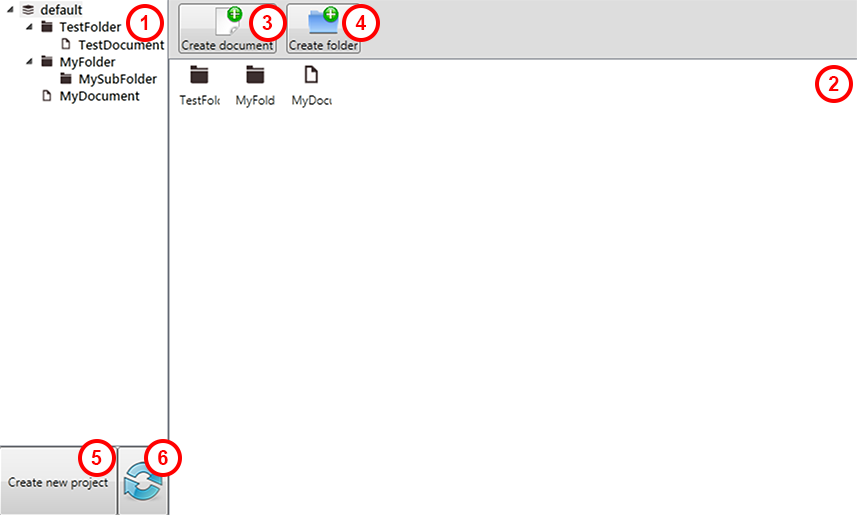
\includegraphics[width=1\textwidth]{User_manual/graphics/local.png}
\caption{Screenshot of the local client}
\end{figure}

\subsubsection{Projects}
Projects are the primary container entity in the program and can can contain folders or documents, but not other projects. You always have at least one project (standard project is called "default").

\paragraph{Create project}
To create a new project, click the Create new project button (5) and enter the desired name in the popup window. You can now find your new project in the explorer (1).

\paragraph{Share project}
In order to share a project in the local client, your data has to be synchronized at some point before, meaning you do not have to have an up-to-date project, folder or document, but the project has to exist online. When this requirement is fulfilled, you can right-click a project in the explorer (1) and click Share project. This will open a popup window with a text field, which can handle both single email addresses or comma-separated email addresses.

\paragraph{Remove project}
To remove a project, right-click the project and click Remove project. Be aware that all folders, subfolder and documents will also be removed.

\paragraph{Synchronize}
To synchronize your data, click the synchronize button (6) and enter your account information in the popup window. If the user does not exist, a new one will be created with the desired account information. All data will then be synchronized, which can take several moments.

\subsubsection{Folders}
\subsubsection{Create folder}
\subsubsection{Remove folder}

\subsubsection{Documents}
\subsubsection{View document}
\subsubsection{Create document}
\subsubsection{Edit document}
\subsubsection{Remove document}
\subsubsection{Show revisions}